\chapter{Analatycs and Requirements specifications}

\section*{Introduction}
This chapter meticulously examines the current environment, including its existing architecture and deployment process. This in-depth analysis will ensure comprehensive coverage of both functional and non-functional needs and requirements. We'll then establish a roadmap for utilizing the Scrum process, defining objectives and deliverables along the way.

\section{Infrastructure Study}
The company is currently using the baseline web application architecture provided by Microsoft\cite{baseline}.
This figure \ref{fig:gloabal_architecture} presents the global architecture of the application.

\begin{figure}[H]
    \centering
    \frame{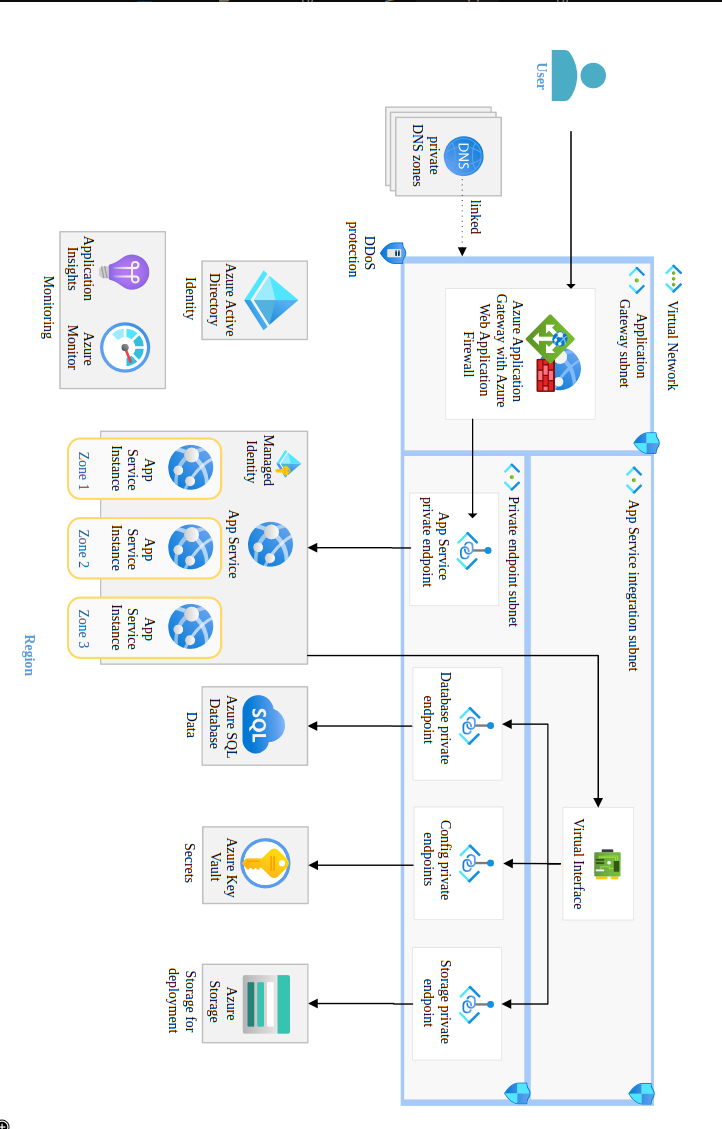
\includegraphics[width=0.8\columnwidth]{gloabal_infrastructure.png}}
    \caption{gloabal architecture}
    \label{fig:gloabal_architecture}
\end{figure}

\pagebreak

\subsection*{\textbullet\ Description}
The architecture exposes a public endpoint via Azure Application Gateway with a Web Application Firewall. The App Service application uses virtual network integration to securely communicate to Azure PaaS services such as Azure Key Vault and Azure SQL Database.

\subsection{Componants of the architecture}
\begin{itemize}
    \item \textbf{Virtual Network:} This is the fundamental building block for your private network in Azure. It provides isolation and protection for your resources.
    \item \textbf{App Service:} This service is used to host the web application. It provides a fully managed platform for building, deploying, and scaling web apps.
    \item \textbf{Azure SQL Database:} This service is used to store the application data. It provides a fully managed relational database with built-in high availability and security.
    \item \textbf{Azure Key Vault:} This service is used to store and manage application secrets. It provides a secure and centralized storage for application secrets.
    \item \textbf{Azure Application Gateway:} This service is used to protect the web application from common web vulnerabilities. It provides a web application firewall and other security features.
    \item \textbf{Azure Monitor:} This service is used to monitor the health of the web application. It provides logging and application telemetry to monitor the health of the application.
    \item \textbf{Azure DevOps:} This service is used to automate the deployment of the web application. It provides a set of tools for building, testing, and deploying applications.
    \item \textbf{Virtual Interface:} This service is used to connect the web application to the virtual network. It provides a secure and private connection to the web application.
    \item \textbf{Application Insights:} This service is used to monitor the performance of the web application. It provides real-time monitoring and analytics for the web application.
    \item \textbf{Private DNS Service:} This service is used to resolve the DNS names of the Azure PaaS services. It provides a secure and private DNS resolution for the web application.
    \item \textbf{Private endpoint:} This service is used to connect the web application to the Azure PaaS services. It provides a secure and private connection to the Azure PaaS services.
\end{itemize}

\subsection{Network flows}
\textbf{Inbound flow:}
\begin{itemize}
    \item The user issues a request to the Application Gateway public IP.
    \item The WAF rules are evaluated.
    \item The request is routed to an App Service instance through the private endpoint.
\end{itemize}
\textbf{App Service to Azure PaaS services flow:}
\begin{itemize}
    \item App Service makes a request to the DNS name of the required Azure service. The request could be to Azure Key Vault to get a secret, Azure SQL Database.
    \item The request is routed to the service through the private endpoint.
\end{itemize}

\textbf{Deploying to the app service:} \\
The deployment process is initiated from the Azure portal by the admin from his machine.

\subsection{Architecture characteristics}
\begin{itemize}
    \item For security reasons, the network in this architecture has separate subnets for the Application Gateway, App Service integration components, and private endpoints. Each subnet has a network security group that limits both inbound and outbound traffic for those subnets to just what is required.
    \item The App Service baseline configures authentication and authorization for user identities (users) and workload identities (Azure resources) and implements the principle of least privilege.
    \item Azure Monitor collects and analyzes metrics and logs from your application code, infrastructure (runtime), and the platform (Azure resources).
\end{itemize}
\section{Deployment Process}
The process of releasing a new application version or update in our system follows a multi-step approach. This approach ensures a smooth transition from development to production and minimizes the risk of introducing issues.
Here's a breakdown of the key stages involved:
\begin{itemize}
    \item \textbf{Code Preparation:} During this stage, developers finalize the code for the new application version or update. This may involve tasks like code reviews, bug fixing, and integration with existing systems.
    \item \textbf{Testing:} Once the code is prepared, it undergoes rigorous testing by the Quality Assurance (QA) team. This testing verifies that the application functions as intended identifies and resolves any bugs or errors, and ensures compatibility with different environments.
    \item \textbf{Deployment Scheduling:} Following successful testing, a deployment plan is created. This plan defines the specific time and method for releasing the application to users. The plan often involves coordination between development, QA, and system administration teams to ensure a smooth rollout and minimal disruption to ongoing operations.
    \item \textbf{Deployment:} During deployment, the application is transferred from its development environment to the production environment where it will be used by end-users. This process may involve tasks like uploading application files, configuring settings, and integrating with databases or other systems.
    \item \textbf{Monitoring:} After deployment, the system administrators closely monitor the application's performance and functionality. This monitoring helps to identify any issues that may arise after the release and allows for prompt intervention if necessary.
\end{itemize}
Effective collaboration between development, QA, and system administration teams is crucial throughout this process. Clear communication and well-defined roles ensure a successful application deployment with minimal downtime and a positive experience for end-users.

\section{Needs and requirements}
To be able to improve the current deployment process while ensure the security and performance of our applications, we have identified the following needs and requirements:
\noindent
\subsection{Functional Needs}
\begin{itemize}
    \item \textbf{Patch Deployment Automation:} Implement a system for automated deployment of patches to applications and systems.
    \item \textbf{Version Rollback Capability:} Provide the ability to revert to a previous version of an application during deployment in case of failure or unexpected issues.
\end{itemize}
\subsection{Non-functional Needs}
\noindent
\begin{itemize}
    \item \textbf{Availability:} Ensure high availability of applications and services, minimizing downtime during deployments.
    \item \textbf{Security:} Implement Web Application Firewall (WAF)) to safeguard applications from cyber threats.
    \item \textbf{Performance:} Optimize deployment processes to maintain optimal performance levels of applications and systems.
    \item \textbf{Cost optimization:} Minimize the costs associated with deployment processes, including recourses and infrastructure.
\end{itemize}

\section{The implementation of Scrum process}
This overview outlines how we will be implementing the Scrum process to manage our project:

\subsection{Scrum Roles}
\begin{longtable}[c]{
    |p{.35\textwidth}
    |p{.35\textwidth}|
    }
    \caption{the key technical objectives for the project}
    \label{tab:Scrum-team}                     \\
    \hline
    Roles          & Members                   \\ \hline
    Scrum Master   & Mme. Yosra najjar         \\ \hline
    Product owner  & Mr. Yazid Missaoui        \\ \hline
    Developer team & Mr. Mohamed ben hadj nasr \\ \hline
\end{longtable}

\subsection{Scrum events}
\begin{itemize}
    \item \textbf{Retrospective (Weekly):} Held with the company supervisor to review the previous sprint, identify areas for improvement, and adapt the process for the upcoming sprint. This meeting can take place in person at the supervisor's office or virtually using Microsoft Teams.
    \item \textbf{Sprint Planning (Before Each Sprint):} Select items from the backlog and commit to delivering them during the upcoming sprint (a short iteration typically lasting 2 weeks).
\end{itemize}

\subsection{Scrum implementation}
\begin{itemize}
    \item \textbf{Product Backlog:} I will maintain a product backlog that outlines all the features and functionalities desired in the final product.
    \item \textbf{Sprint Planning:} Before each sprint, a sprint planning meeting is held by the supervisor and me to select a set of items from the top of the product backlog that we commit to delivering during the upcoming sprint. This selection is called the sprint backlog.
    \item \textbf{Sprint Execution:} I deliver the items in the sprint backlog. with each sprint lasting two weeks.
    \item \textbf{Sprint Retrospective:} At the end of each sprint, I will hold a sprint retrospective meeting with the company supervisor. This meeting will focus on reviewing what areas need improvement in the upcoming sprint.
\end{itemize}

\subsection{Product backlog}
By analysing the needs and requirements, we have defined the following product backlog that will be provided during multiple sprints:
\begin{longtable}[c]{
    |p{.05\textwidth}
    |p{.85\textwidth}|
    p{.1\textwidth}|
    }
    \caption{the key technical objectives for the project}
    \label{tab:productBacklog}                                                                          \\
    \hline

    num & epics                                                                                & effort \\ \hline

    1   & Define the structure and variables for the web Terraform module                      & 4 days \\ \hline
    2   & Define the structure and variables for the database Terraform module                 & 4 days \\ \hline
    3   & Define the structure and variables for the storage account Terraform module          & 2 days \\ \hline
    4   & Implement the DNS zones for each module and set up the connections between them.     & 4 days \\ \hline
    5   & Configure security groups for resources in each module.                              & 1 days \\ \hline
    6   & Define environment-specific variables for the rest of the environments: QA and prod. & 4 days \\ \hline
    7   & Deploy a simple web application to test the infrastructure.                          & 1 days \\ \hline
    8   & write the necessary documentation on how to use the different workspaces.            & 2 days \\ \hline
    9   & Test connectivity between the web application and the database for each environment. & 3 days \\ \hline
    10  & Configure the production environment for optimal performance.                        & 2 days \\ \hline
    11  & research the different branching strategies and pick the appropriate one.            & 2 days \\ \hline
    12  & create the build pipeline and publish the artifacts for each environment.            & 4 days \\ \hline
    13  & create the provisioning pipeline for the development environment                     & 4 days \\ \hline
    14  & set up the management of the state file of the terraform in the pipeline             & 2 days \\ \hline
    15  & create the release pipelines for the staging and production environments             & 3 days \\ \hline
    16  & test the pipeline by pushing code to the different branches and checking the results & 2 days \\ \hline
    17  & research the different deployment strategies and select the most appropriate one     & 3 days \\ \hline
    18  & research the different rollback strategies and select the most appropriate one       & 3 days \\ \hline
    19  & compare the different ways to implement the deployment strategy.                     & 2 days \\ \hline
    20  & implement the deployment strategy in the production release pipeline                 & 4 days \\ \hline
    21  & implement the rollback strategy in the production release pipeline                   & 4 days \\ \hline
    22  & test the downtime of the deployment during an update.                                & 2 days \\ \hline
    23  & test the rollback procedure.                                                         & 2 days \\ \hline
\end{longtable}

\subsection{Definition of Done}
The definition of done is a checklist of requirements that must be met before a task can be considered complete.

\begin{itemize}
    \item the deployment must be done with no manual intervention.
    \item the production environment must not be dowm for more than 3 minutes during the deployment.
    \item the rollback procedure must be tested and working in under than 4 minutes.
    \item commits in the dev branch must result in the creation of a new testing environment.
    \item the infrastructure must provisioned in a maintanable and reproducible code.
\end{itemize}

\subsection{Sprint planning}
sprint planning can be found in the gantt diagram below:

\begin{figure}[htbp]
    \centering
    \frame{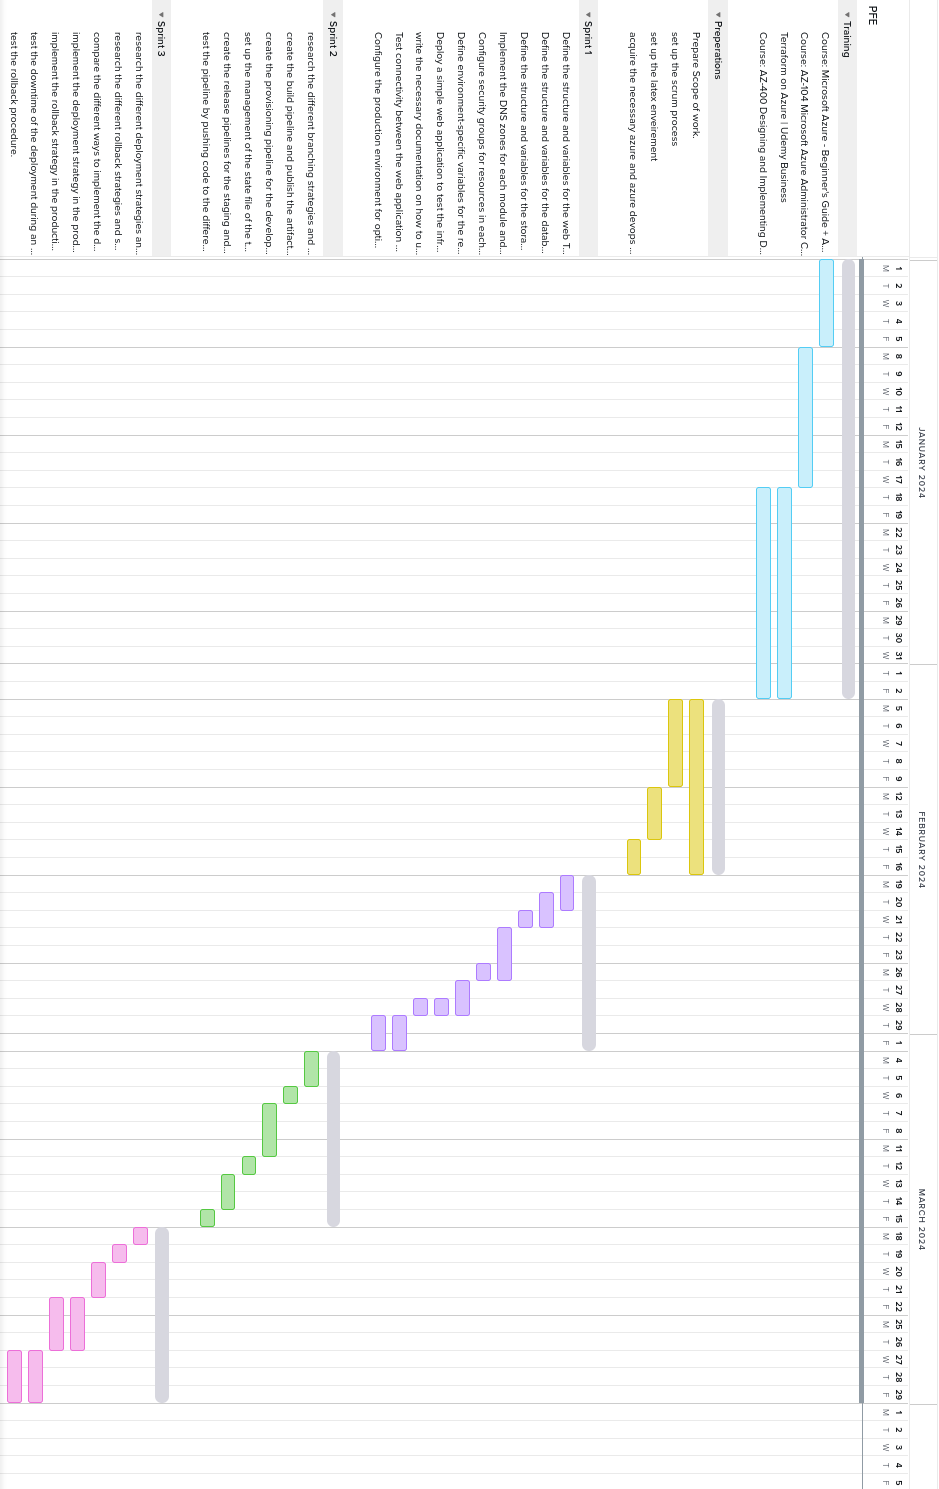
\includegraphics[width=0.9\columnwidth]{gantt.png}}
    \caption{This is the gantt chart of the scrum process}
    \label{fig:gantt_chart}
\end{figure}

\section{Description of available tools}

\subsection{Terraform}

\begin{figure}[H]
    \centering
    \frame{
\includegraphics[width=0.5\columnwidth]{Terraform.png}}
    \caption{Terraform}
    \label{fig:terraform}
\end{figure}

Imagine building your software on a foundation pre-designed with specific instructions, rather than individually placing each brick. This is the essence of Terraform, an open-source IaC tool. It allows you to define the infrastructure your application needs using a simple language, similar to writing instructions. This simplifies managing resources across different environments (cloud-based or on-premises) with consistent configurations, ensuring everything is built according to your specifications.
\par
\textbf{Alternatives:}
\begin{itemize}
    \item \textbf{Azure Resource Manager (ARM) templates:} These templates are native to Azure, offering familiarity and direct management within the platform. However, they require more technical knowledge and lack the flexibility and reliability of IaC tools like Terraform.
    \item \textbf{Bicep} Think of Bicep as a specialized architect fluent in Azure, Microsoft's cloud platform. It speaks Azure's language directly, making it easier to design and manage resources within that specific environment. However, since its expertise is limited to Azure it does not have the community support offered by an open-source project like Terraform.
\end{itemize}
By understanding these factors, we can make the informed decision that the IaC tool that best suits our requirements is Terraform.
\subsection{Azure DevOps}

\begin{figure}[H]
    \centering
    \frame{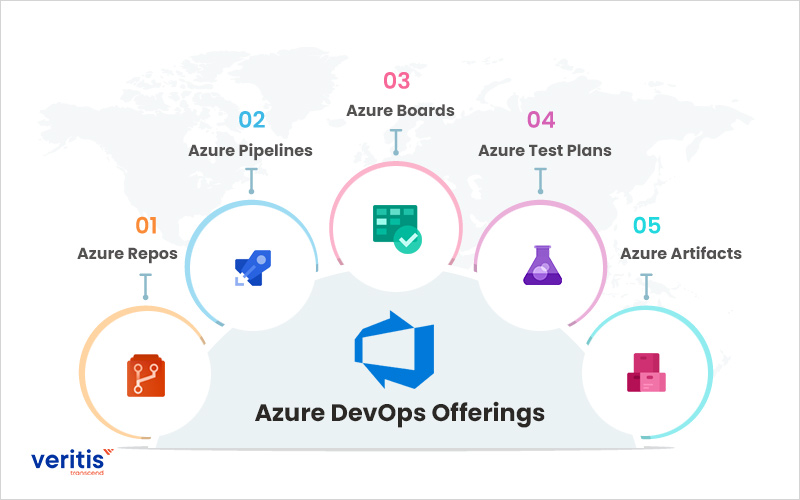
\includegraphics[width=0.5\columnwidth]{azure-devops-offerings.jpg}}
    \caption{Azure DevOps}
    \label{fig:Azure_DevOps}
\end{figure}

This platform acts as a comprehensive toolkit for software teams, offering various features to manage the entire development lifecycle efficiently.
\par
\textbf{Features:}
\begin{itemize}
    \item \textbf{Azure Repos:} This feature keeps your code organized and secure, just like a well-structured library holding all your project versions. It can use either Git or Team Foundation Version Control (TFVC) to manage your code.
    \item \textbf{Azure Pipelines:}  This service automates tasks like compiling code, running tests, and deploying new versions, saving time and minimizing errors.
    \item \textbf{Azure Boards:} Planning and tracking progress becomes transparent with this feature. It provides Kanban boards visually displaying tasks, backlogs listing upcoming work, and sprint planning tools.
    \item \textbf{Azure Artifacts:} Sharing reusable components becomes effortless with this feature. Think of it as a shared storage space for code modules, containerized applications, and other resources your team can easily access and reuse across projects.
\end{itemize}

\section*{Conclusion}
This chapter's comprehensive analysis of our cloud environment, infrastructure, and deployment process provides a firm foundation for the next crucial step: constructing a secure, efficient, and automated cloud-based deployment framework. With this groundwork laid, we can confidently transition to the realization phase, detailed in the next chapter, where we'll navigate the provisioning of our current infrastructure.
